%!TEX root = ../thesis.tex
%*******************************************************************************
%****************************** Third Chapter **********************************
%*******************************************************************************
\chapter{Discussion}

% **************************** Define Graphics Path **************************

\graphicspath{{Chapter5/Figs/Vector/}{Chapter5/Figs/}}


\section{Non-Parametric}
Three algorithms tested of non-parametric variety producing several noticeable results. Firstly, the baseline result did not produce the worst results with respect to accuracy, although precision was consistently worse. This is demonstrated convincingly through Figure~\ref{fig:nPComp} where results from the greedy results suggest the worst accuracy.

Despite the greedy algorithm demonstrating the worst accuracy, interesting results were shown with ROD sampling. Indeed, the progression from the first to the second and third iteration demonstrates a faster average learning rate than the other algorithms. This is expected as the ROD algorithm specifically targets regions of the model which are challenging causing the largest changes towards proper fitting.

Both ROD and greedy sampling are suspected to suffer from clusterisation whereby data points similar to each other in the feature space are sampled within the same batch, thus reducing the total information conveyed per batch operation. The random nature of Monte Carlo reduces this prospect, hence the apparent promising performance of a random sampling methodology.

\begin{figure}[h]
    \begin{center}
        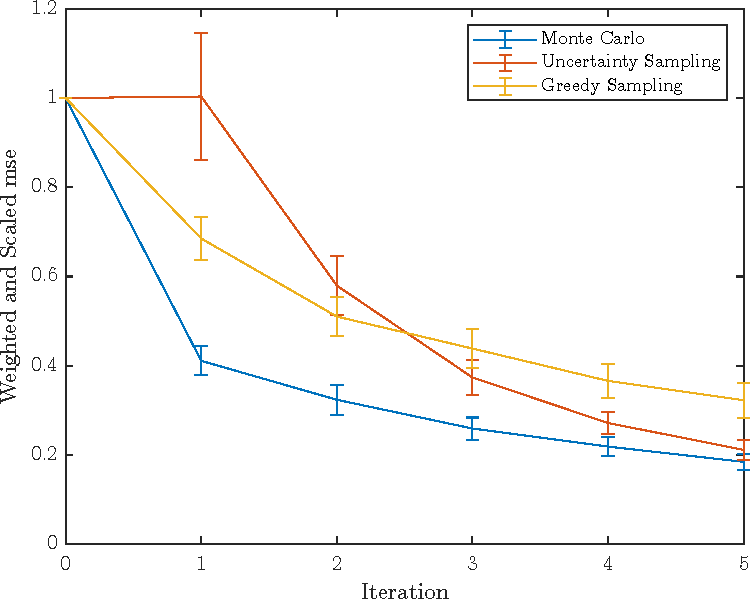
\includegraphics{nonParamComp1.pdf}
        \caption[Non-parametric comparison]{Comparison of different non-parametric algorithms with standard deviations represented as error bars.}
        \label{fig:nPComp}
    \end{center}
\end{figure}

\section{Parametric}
\blindtext[3]

